\documentclass[a4paper]{article}

\usepackage[english]{babel}
\usepackage[utf8]{inputenc}
\usepackage{amsmath}
\usepackage{graphicx}
\usepackage[colorinlistoftodos]{todonotes}

\newcommand{\figref}[1]{Fig.~\ref{fig:#1}}

\title{Model-based Closed-loop Validation of Medical Devices}

\author{You}

\begin{document}
\maketitle

\begin{abstract}
Your abstract.
\end{abstract}

\section{Closed-loop Medical Devices}
Most medical devices operate with the patient in certain closed-loop manner. For diagnose-only devices, i.e. the X-ray machine, the physician operates the device to obtain patient data, perform diagnosis and deliver proper therapy to the patient (\figref{closed-loop}.(a)). For therapy-only devices, i.e. the infusion pumps, the physician operates the device to perform therapy on the patient according to previous diagnosis (\figref{closed-loop}.(b)). We denote these devices as \textbf{Open-loop Medical Devices} as there is no direct closed-loop interaction between the device and the patient. For open-loop devices, the safety of the patients is mostly guaranteed by the professionally-trained physicians in the loop. Device safety focus on providing accurate information to the physicians and faithfully operate as instructed by the physicians.

Among all the medical devices, there are devices with both diagnostic and therapeutic functions, i.e. implantable cardiac devices to treat cardiac arrhythmia, deep brain stimulation devices (\cite{Brain_sti}) to treat Parkinson's disease and artificial pancreas to treat Type 1 diabetes\footnote{The artificial pancreas is till under development by \cite{}}. These devices diagnose physiological conditions of the patient using sensory data, and deliver therapy accordingly (\figref{closed-loop}.(c)). These devices usually operate (semi-) autonomously with very little human intervention, thus malfunctions or inappropriate therapies from these devices cannot be corrected timely, which can cause serious adverse effects on patients' health. Therefore these devices are usually classified into the highest risk category and undergo the most stringent regulation. We denote them as \textbf{Closed-loop Medical Devices}. 
\begin{figure}[t]
		\centering
		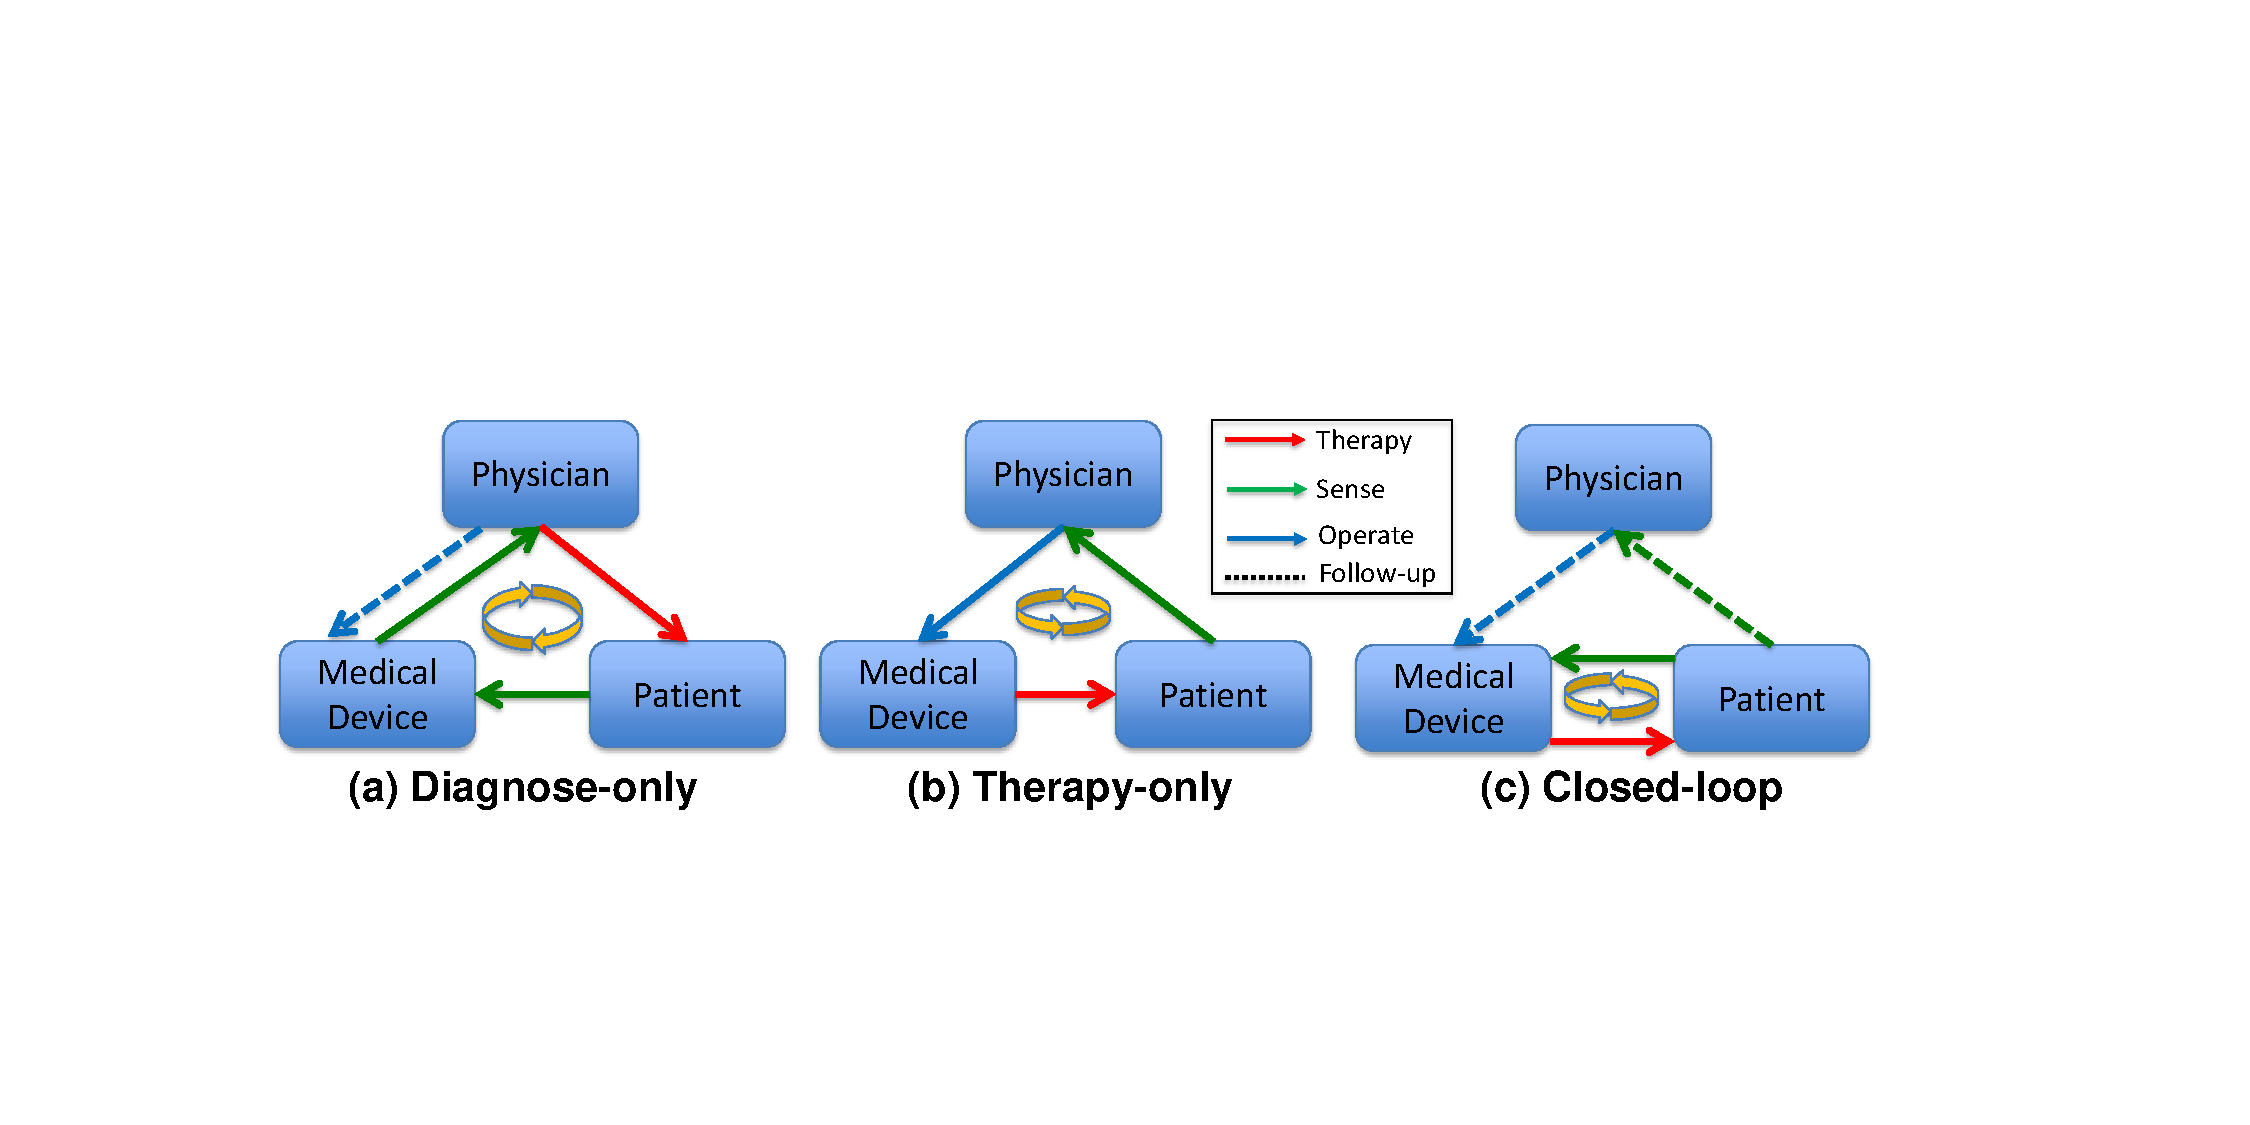
\includegraphics[width=\textwidth]{figs/closed-loop.pdf}
		\caption{\small Closing the Loop With the Patient}
		\label{fig:closed-loop}
\end{figure}
There are multiple challenges to develop safe and effective closed-loop medical devices:

\textbf{Closed-loop Interactions With Complex Physiology}\\
When using open-loop medical devices, the diagnosis and therapy decisions are made by medical professionals, who has abundant knowledge of human physiology. Therefore they are able to identify adverse health conditions and adjust the therapy accordingly. On the other hand, closed-loop medical devices have to make both the diagnosis and therapy decisions on their own. The domain expertise required to make those decisions has to be programmed into the device. It is impossible to encode all the knowledge of human physiology into the device. Therefore when conditions happen and are not programmed into the device, the device may deliver inappropriate therapy which can cause adverse effect on patient's health. 

With the development of new technology, new therapies to certain disease may arise and adopted by closed-loop devices. Certain closed-loop interactions between the device and the human physiology may not be well-understood, even to the medical professionals. Combinations of well-understood behaviors may also be the source for inappropriate therapies. 

\textbf{Limited Diagnostic and Therapeutic Functions}\\
One fundamental rationale behind closed-loop medical devices is to enable the patients to live their normal lives without the dependance of cumbersome medical devices and/or the supervision of physicians. In fact, a large number of closed-loop medical devices are implantable devices. As a result, the sensing and therapy capabilities of the devices are limited, in order to increase portability and reduce invasiveness. Limited sensing capabilities may cause inaccurate diagnosis and therefore inappropriate therapy, as multiple conditions can map to the same sensor inputs. Due to limited therapy capabilities, there exists sub-optimal physiological conditions that are untreatable. The device may even trigger the conditions into less optimal conditions. 

\textbf{Heavy Reliance on Software Control}
Due to the complexity of the diagnostic and therapeutic functions of the closed-loop devices, these functions are mostly controlled by their software components. 
Software embedded in a medical device, unlike electrical and mechanical components, does not fail due to corrosion, fatigue or have statistical failures of subcomponents. Software failures are uniquely sourced in the design and development of the system. %Unlike other industries such as consumer electronics where product life cycles are measured in months, software engineering for medical devices often spans a decade and must prioritize safety and efficacy over time to market. 

%  Over the course of the past four decades, cardiac rhythm management devices such as pacemakers and implantable cardioverter defibrillators (ICD) have grown in complexity and now have more than 80,000 to 100,000 lines of code (\cite{pauljones}). 
According to the US Food and Drug Administration, in 1996, 10\% of all medical device recalls were caused by software-related issues (\cite{medstats}). This percentage rose to an average of 15\% of recalls from 2008 to 2012 (\figref{soft_recalls}). Malfunctions of closed-loop medical devices usually have severe consequences, which will be categorized as \emph{Class I}, meaning there is a ``reasonable probability that use of these products will cause serious adverse health consequences or death.'' (\cite{medstats2,pacemakerrecalls,killedbycode}). 
	
\begin{itemize}
	\item What are the differences between closed-loop medical devices vs. open-loop medical devices (Interact directly in closed-loop with physiology, With/without physician intervention)
	\item Example closed-loop medical devices (Pacemaker/ICD, deep brain stimulation, artificial pancreas, autonomous infusion pump)
	\item What are the challenges for closed-loop medical devices (interaction with physiology, limited capability, reliance on software)
	\item The need for closed-loop evaluation and the insufficiency of clinical trials as the only closed-loop evaluation method
\end{itemize}

\section{Computational Models for Physiological Behaviors}
Closed-loop validation of medical device
\begin{itemize}
	\item As example ,show list of different computational models of the heart (electrical, mechanical, anatomical)
	\item What are their applications? (understand mechanisms, predictions)
\end{itemize}

\section{Physiological Models for Closed-loop Evaluation of Closed-loop Medical Devices}
Model simulation results are accepted by FDA as safety evidence (Artificial pancreas)
\begin{itemize}
	\item Key characteristics for interaction with closed-loop medical devices (interface, distinguish conditions, interpretation of execution traces, identifiability)
	\item Why do aforementioned models not suitable for evaluating devices? (unnecessarily complex)
\end{itemize}

\section{Model-based Closed-loop Evaluation of Closed-loop Medical Devices}
Enable closed-loop validation earlier in the development process.
\begin{itemize}
	\item Two applications: Closed-loop Model checking and MBCT
	\item How do they fit into regulation framework

\end{itemize}

\subsection{Closed-loop Model Checking}
Can be used to identify known and unknown mechanisms that can induce hazards.
\begin{itemize}
	\item  Model considerations
	\item Device interface
	\item Coverage vs. Expressiveness
	\item Model refinement
\end{itemize}

\subsection{Model-based Clinical Trials}
Cover target population

\begin{itemize}
	\item Modeling considerations
	\item What is clinical trials and what can they achieve?
	\item What clinical trials cannot achieve? (\textbf{reproducibility}, large population)
	\item How can MBCT help?
\end{itemize}
\bibliographystyle{plain}
\bibliography{bibliography}
\end{document}